\documentclass[11pt]{article}
\usepackage{natbib} % our bibliography system 
\usepackage{graphicx} % allows graphics
\usepackage{hyperref} % for adding color and clickable links to references

% configuration of {hyperref} package
\hypersetup{
  colorlinks=true,
  linkcolor=blue,
  citecolor=blue,
  urlcolor=blue
}

\usepackage{amsmath} % allows numbered equations, for one thing
\usepackage{authblk} % to add more authors

\usepackage[a4paper, total={6in, 8in}]{geometry}

\usepackage[dvipsnames]{xcolor} % adds 68 named colors and the ability to define your own, but can cause trouble with beamer and tikz; tikz must be declared after this

\usepackage{mathpazo} % URW Palladio, from Palatino
\usepackage{microtype} % cleans up the kerning and hypenation
\usepackage[margin=15pt,font=small,labelfont={bf}]{caption} % cleans up the structure of the captions

\usepackage{mdframed} % for framed text boxes; does not play well with lineno

% frame style
\mdfdefinestyle{textBox}{%
  linecolor=boxLine,
  outerlinewidth=2pt,
  roundcorner=20pt,
  innertopmargin=-6pt,
  innerbottommargin=10pt,
  innerrightmargin=4pt,
  innerleftmargin=4pt,
  leftmargin = 2pt,
  rightmargin = 2pt,
  backgroundcolor=boxBG
}


\renewcommand\Affilfont{\small}

\title{Inheritance, Ecology and the Evolution of the Canoes of East Oceania}
\author[,    1]{Bret A. Beheim\footnote{Corresponding author. babeheim@ucdavis.edu}}
\author[1]{Adrian V. Bell}

\affil[1]{Graduate Group in Ecology, Department of Environmental Science and Policy, University of California, Davis, USA}
\date{26 January 2011}

\begin{document}

\setlength{\parindent}{30pt}

\maketitle

\begin{center}
{\bf Keywords:} cultural evolution, Polynesia, canoes, model selection, DIC
\end{center}

\begin{abstract}
We consider patterns in the evolution of canoe technology in the eastern Pacific relative to three general processes: movement of canoe traits along the Polynesian settlement sequence, adaptations to local island environment, and post-settlement interaction between island groups. Using model selection methods on the distributions of canoe technology, we show that social and ecological covariates together consistently outperform each considered individually, though knowledge of island area and post-settlement trading spheres does not add explanatory power. In particular, decorative canoe traits are not effectively explained by either our ecological or transmission models. We also estimate negative effects from both settlement sequence and island geomorphology consistent with the die-off of particular canoe designs on resource-rich high island groups such as Hawaii and New Zealand. This decline in measured traits may be due to the lifting of ecological constraints on population size or building materials.
\end{abstract}

\section{Introduction}

Anthropologists have long debated the relative influence of cultural inheritance and ecological adaptation on the evolution of a society's social, technological and institutional forms. Historically-minded social scientists stress the entrenching effects of the social reproduction of culture, which allow cultural continuity over time and provide the defining structures of society \citep{Gaddis2002, wimsatt2007reproducing}. Both theoretical modeling and empirical analysis have indicated that idiosyncratic aspects of a society's technological and behavioral repertoire do indeed persist across time and space, plausibly due to processes of cultural transmission that resist innovation \citep{Edgerton1971,Guglielmino1995, Nisbett1996, Richerson2005, eerkens2017cultural, Temkin2007:CulturePhylogenetics}.

Others, however, favor the simplifying premise that human behavioral adaptation can occur quickly enough to be seen as a product of a group's contemporary ecological environment \citep{Steward1955, Diamond2002domestication}. An environment's climate, availability of potable water, mineral resources, and domesticable animals and plants may significantly constrain or influence socio-political systems \citep{johnson2000evolution, Kirch2007}, regardless of their particular cultural histories or neighbors \citep{rogers1997phylogenetic, cashdan1997human}. In problems of reproductive investment and subsistence strategies, humans appear to regularly maintain near-optimal behavior with respect to their inclusive fitness, providing support for the ``phenotypic gambit'' \citep{WinterhalderSmith2000}. 

While some form of cultural transmission or scaffolding is obviously necessary for any technological continuity in space or time, adaptation to a local environment may be fast  enough that a society's particular history or larger social context does not meaningfully add to our understanding of its configurations. Conversely, if historical entrenchment or the influence of trade networks are pronounced, a society's ecological context may have very little to do with its forms of material culture. Despite the importance of these hypotheses to social science, and decades of sometimes polemical debate about what matters and what does not \citep{Harris1968, Sahlins1976:critiqueSociobiology,Betzig1997humannature}, the relative importance of these influences remains poorly understood. Using methods from information theory, we formalize these alternatives as statistical models and apply a model selection analysis to patterns of material variation in the canoe designs of Polynesia and Fiji. This approach allows us to quantify the relative explanatory benefits of situating a society within its historical, social and ecological context when studying an observed pattern of cultural variation.

\subsection{Canoe evolution in Polynesia \& Fiji}  

Pacific societies have attracted generations of anthropologists and ecologists for their ability to serve as natural ``laboratories'' of human behavior and socio-ecological processes \citep{Mead1957:PolynesianLab}, and are particularly useful for testing models of cultural transmission and behavioral ecology. Although the peopling of the Pacific has captured the attention of centuries of scholarship, debates continue about (a) how purposive Polynesian voyaging was \citep{Whyte2005:PolyHumanEvol}, (b) the sequence and methods of settlement \citep{Irwin1992}, (c) how quickly it occurred \citep{Anderson2000:Slowboats, Thomas2008:Lastpulse, Gray2009:Phylogenies}, (d) the extent of pre-European trade and interaction  \citep{Weisler1998}, (e) the kinds of canoes and sailing rigs employed in these activities \citep{Doran1981canoes, Anderson2001:SharpEnd}, and (f) the evolutionary processes that shaped them \citep{Horridge1987:IndonesiaCanoes}. Apart from the written accounts of Europeans, very little information is known about the canoe technology of pre-contact Polynesia. In the early twentieth century, A.C. Haddon and James Hornell compiled the three-volume \textit{Canoes of Oceania} from available written accounts and their own field observations, a work that still remains the authority on Polynesian seacraft \citep{HaddonHornell1936}.

A recent paper \citep{Rogers2008:Canoes} uses data extracted from this source to argue that the diversity in canoe design observed across Fiji and Polynesia was likely shaped by differential viability selection: canoe components vital to successful voyaging experienced strong negative, stabilizing selection pressures, while decorative traits were less constrained and changed more rapidly over time. The authors use the descriptions of the canoes on eleven different Pacific archipelagos in \textit{Canoes of Oceania} to measure the relative amount of change in canoe technologies via a table of presence-absence data for 134 distinct canoe traits, classified as either ``symbolic'' or ``functional''. They demonstrate that functional components of canoes are significantly more similar across archipelagos than decorative canoe traits, as measure by Jaccard distance matrices.

These results have been criticized as ambiguous \citep{Skoyles2008:canoechange}; a ``significant'' difference between the two subsets of canoe traits may be due to negative selection pressures but is consistent with any number of random or directional processes, only a few of which support an evolutionary selection hypothesis. 

Because aggregate historical data are often unsuitable for distinguishing between particular processes of cultural change, we instead attempt a pattern-centric analysis which contextualizes the canoe data, and can identify general characteristics of the causal evolutionary forces even as they remain unknown. Specifically, by situating canoe designs within their ecological and social milieu, we ask which factors in an archipelago's local environment, settlement history, and regional trade networks best predict the observed trait variation. This contextualizing, empirically rich approach is also applied to the dataset; we have extensively modified the \cite{Rogers2008:Canoes} canoe traits, merging or excluding them based on the practical details of canoe design (see ESM for details). 

\section{The Model Selection Approach}
 
While popular, many standard null-hypothesis tests were initially developed in the early twentieth century for the analysis of randomized, controlled experiments, and their limitations are well-documented \citep{Berger1988, Cohen1994, Anderson2000hull}. Recent advances in statistical methodology have produced methods better suited for observational data, and as a result are becoming extensively used in field ecology and evolutionary biology \citep{Hilborn1997, Johnson&Omland2004:modelselection, Bolker2008}. This methodology does not attempt to measure the probability of seeing data given an assumed model, nor does it employ arbitrary cutoffs to decide which estimates are ``significant'', so as a result there are no $p$-values.

Instead, the focus shifts to measuring which model represents the closest approximation of the processes behind the data \citep{Burnham&Anderson:2002}. Information-theoretic methods attempt to measure the amount of information lost by approximating an infinite-dimensional reality with a model of finite dimensions, by ranking models based on their information-criterion scores.

Rather than construct a single model aiming for ``significant'' covariates, the challenge then shifts to developing several plausible models that embody a diversity of potential hypotheses, and using the model selection framework to test them simultaneously. An often-used analogy is a horse race: while it is sometimes possible to distinguish the best performing horse after a single race, with several close competitors it would be premature to proclaim the winner of one particular race the fastest. Similarly, the particularities of one sample of data may be responsible for one model ranking marginally higher than several close competitors, when in fact they all may be reasonable approximations and should be reported together. Thus, rather than attempt to argue for or against a single hypothesis, our focus shifts to evaluating multiple hypotheses simultaneously.

\subsection{Models of Cultural Inheritance}

\begin{figure}[t]
  \begin{center}
    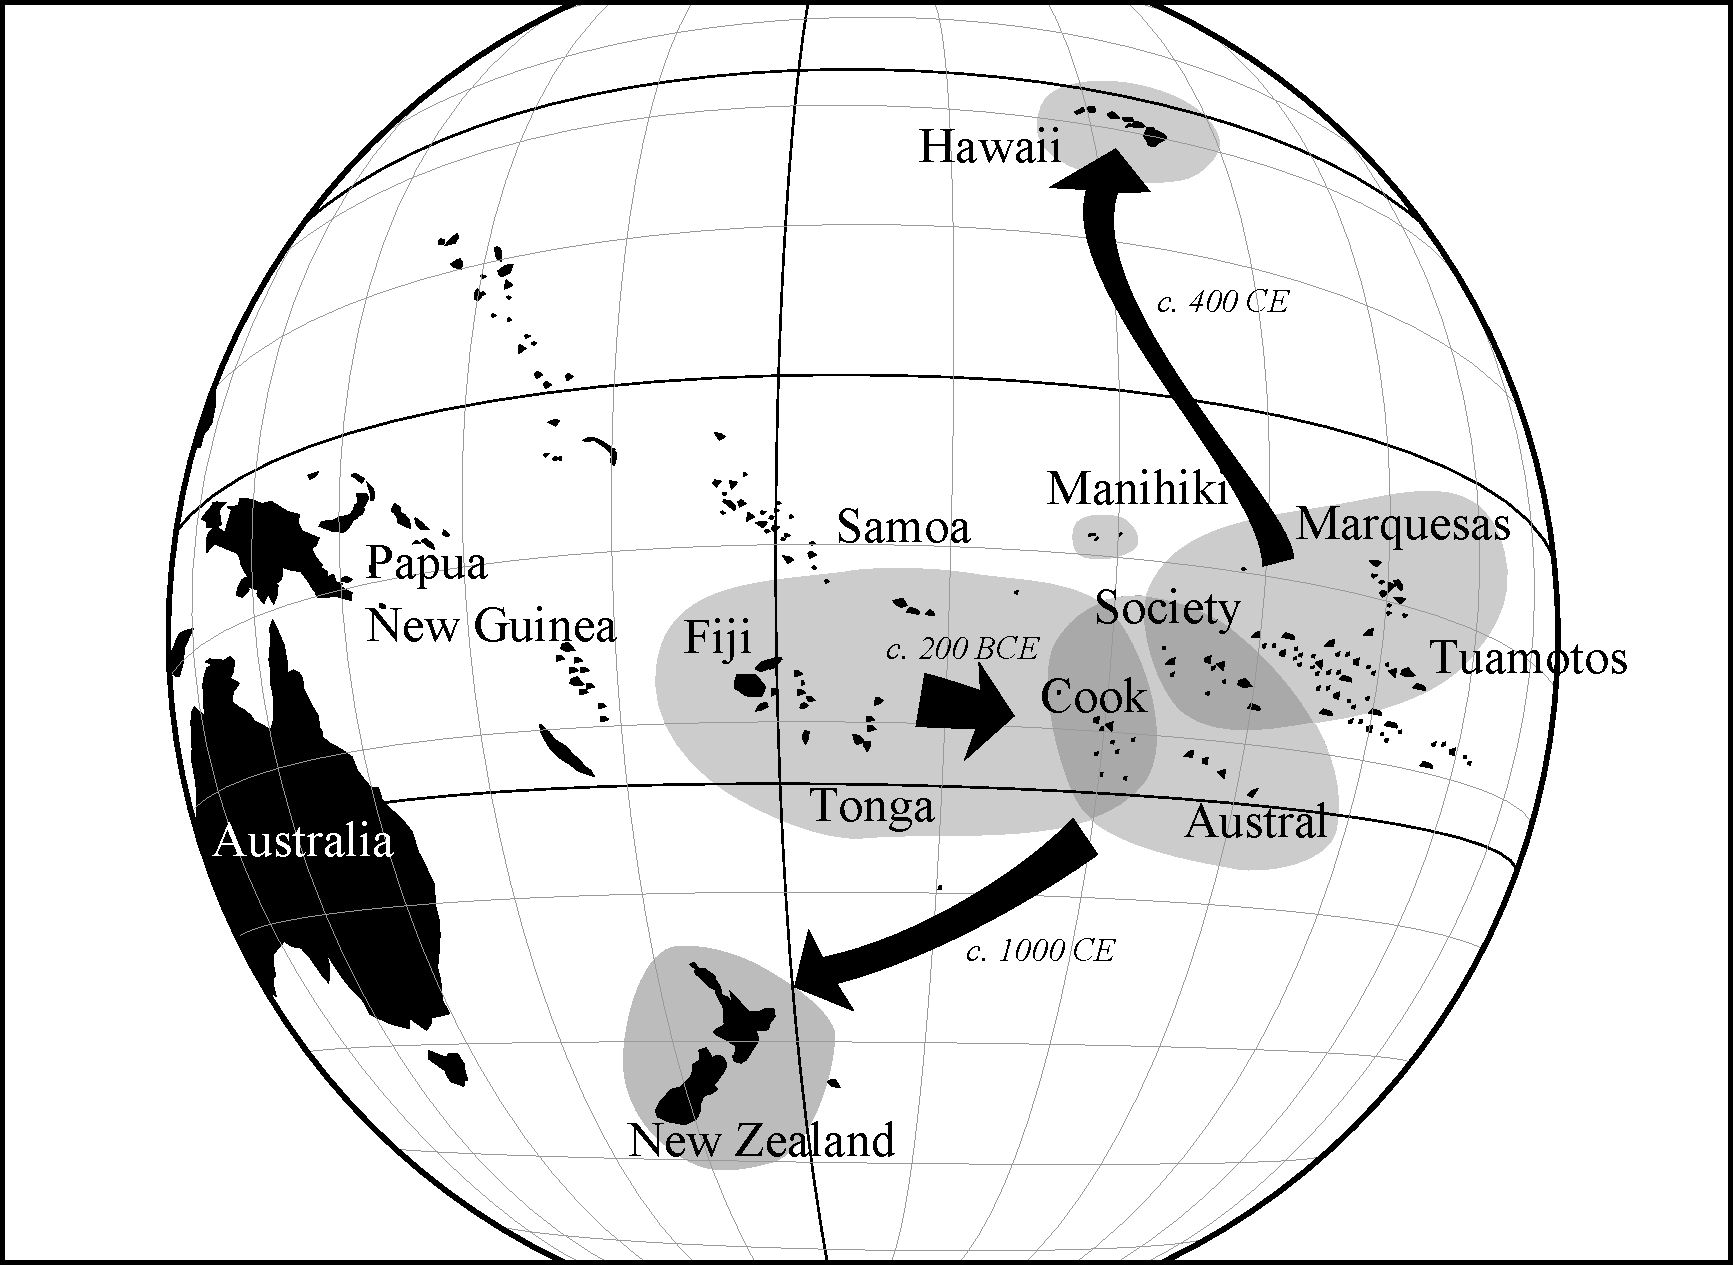
\includegraphics[scale=0.4]{figures/map.pdf}
  \end{center}
  \caption{\small Settlement sequence following \cite{Kirch2000:Road} (black arrows) and five major post-settlement interaction spheres (shaded regions) based on \cite{Weisler1998} in the eastern Pacific.}
  \label{fig:map}
\end{figure}

Our models of Polynesian cultural inheritance focus on two forms of transmission: the inheritance of material culture via colonization, and the flow of information and material technology between established island societies. Given that the exact island-to-island settlement sequence of Polynesia is still contested \citep{Kirch2000:Road, RogersFeldmanEhrlich2009}, we define it in broad, regional generalizations (Figure \ref{fig:map}, black arrows). Currently, it is established that the Polynesian settlers moved west to east through four major regions: first, the triangular region defined by Fiji, Samoa and Tonga, then onto the Cook, Society, Tuamotos, and Austral archipelagos making up Central Polynesia, and from there north to Hawaii and southwest to New Zealand. Broadly speaking, these four regions can be considered a settlement sequence, and so canoe designs in one region may help predict canoe designs in the next region in the sequence. Hawaii petroglyphs, for example, indicate that the Hawaiian crab-claw sail has a common ancestry with the Tahitian analog, and so knowledge about Tahitian canoes should presumably inform us about Hawaiian designs as well \citep{Lewis1978:PacificNavigators}.

Post-settlement interactions between archipelagos also clearly played a role in shaping canoe designs. The Fijian \textit{ndrua} double canoe, described by Haddon and Hornell as the ``largest and finest sea-going vessel ever designed'' in the Pacific, incorporated a shunting-capable rig\footnote{Shunting is an innovation for sailing against the wind unique to Oceanic seacraft in which the rigging is reversed so the fore becomes the aft and vis versa. See ESM for details.} from nearby Micronesia and in turn was the basis for the Tongan \textit{kalia} design and the Samoan \textit{'alia} design \citep[pg.~319]{HaddonHornell1936}. Canoe diffusion was often very direct - Haddon and Hornell report that Society islanders would employ Tuamotoan canoe builders, who in turn imported Tahitian hulls \citep[pg.~74,79]{HaddonHornell1936}. \cite{Weisler1998} presents evidence for six major interaction spheres in the South Pacific, defined by tracing basalt adzes back to their islands of origin using x-ray florescence techniques. Using Weisler's geochemical diffusion data as a guide, we group the islands in our dataset into five general zones of interaction within which canoe technology might have been regularly shared (Figure \ref{fig:map}, shaded regions). Both inheritance from trading spheres and the island-to-island phylogenetic settlement sequence are included as covariates (see ESM for specifications of each).


\subsection{Models of Ecology}

We must also consider the possibility that two societies will resemble each other simply because they exist in similar ecological environments, regardless of whether they interact with each other or share common ancestors. As Kirch describes the experience of migrating Polynesians, ``Whether the new land was too isolated to maintain contacts with the homeland, whether it was vast or small, high or low, endowed with permanent streams, and so on, were factors that were to channel evolutionary pathways in certain directions.'' \citep{Kirch1984evolution}. Canoe builders may converge on hull designs again and again because of ecological pressures or the availability of certain critical resources. For example, islands with protective reefs or atolls with enclosed lagoons allowed for relatively simple dugout designs with low freeboard, while open-ocean canoes necessitated raised washstrakes and weather screens. The narrow Polynesian timber available for basic dugout canoe construction was easily capsized, and for anything but the calmest seas required a secondary stabilization mechanism in the form of an outrigger float or second hull. Once Polynesians reached New Zealand, though, larger trees obviated the outrigger and double hull designs, both of which disappeared altogether after the cessation of regular long-distance voyaging. Astronomical wayfinding techniques were lost, and Maori terminology specific to outrigger construction was either abandoned or repurposed to describe single-hulled Maori designs \citep{Biggs2006}.

The above motivates a number of ecological covariates. Because the geological histories of island chains are effective proxies for many other ecological differences between Polynesian archipelagos \citep{Kirch2000:Road}, the elevation profile of an island (atoll, high island, or the coral-uplift \textit{makatea} island) and the presence or absence of a reef are included as ecological covariates. Island area can be interpreted as a proxy for natural resource availability \citep{Banack1991ethnobotany}, the degree to which its inhabitants relied on trade with other islands for vital supplies, as well as a low-resolution measure of population density and carrying capacity.\footnote{The large size of both Hawaii and New Zealand provide dramatic examples of the effect of area on population size. Even though New Zealand is more appropriately seen as a small continental remnant of Gondwana, we classify it as a high island because its elevation gradients bring similar advantages to the mountainous volcanic islands for canoe technology, such as more diverse and abundant plant and mineral resources.}  Ecological data were collected from descriptions in \cite{MuellerDombois1998vegetation} and through a cross-Oceanic survey using satellite images from Google Earth.

\subsection{Model Specification and Estimation Using Bayesian Statistics}

Using these ecological and cultural covariates, we specified 27 logistic regression models to compare using model selection techniques, divided into four broad categories: null models (N), models incorporating cultural inheritance (C), ecology (E), or both (CE, see the ESM for the details of model specification). The large number of models reflects the fact that environmental and cultural inheritance predictors can influence canoe design in many ways; there is no general theory constraining the structure of these models.

If $i \in {1,2,\dots ,11}$ indexes island group and $t \in {1,2, \dots , 65}$ indexes canoe traits, then the binary variable $x_{t,i} \in \{0,1\}$ describes the presence or absence of trait $t$ on island group $i$ for the 65 $\times$ 11 matrix of island traits $X$. Since the goal is to predict $x_{t,i}$, the general form of each model is
\[
  \mathrm{Logit} \Pr( x_{t,i}=1 ) = \alpha_t + Z_i B,
\]
where $Z_i$ is a vector of ecological and cultural inheritance covariates for island $i$ and $B$ is a vector of coefficients. We know beforehand that different traits likely do not occur with the same baseline frequency (the intercept in a logistic regression model), so we need to estimate a frequency, $\alpha_t$, for each trait (see ESM Table 2). The need to model variation in a large number of traits suggests a model with a large number of parameters, yet the number of island groups represented is relatively small. The classic frequentist approach is unsuitable under these conditions because there is too little data and consequently too few degrees of freedom to fit a large model. We solve this problem by using a single prior distribution for all $\alpha_t$, resulting in models containing 1 to over 150 parameters. This allows us to make a relatively parsimonious model for baseline frequencies, yet permits frequencies to vary across traits.

Because little or no prior information is available, we assign Gaussian priors with high variances to all parameters. The prior for $\alpha_t$ has a mean of zero and a variance of 10, whereas all other parameters have prior variances of 100 (see Box~1 in the ESM for common terms in Bayesian statistics). Using a Gibbs sampler implemented in the software \texttt{R} and \texttt{Winbugs}, we estimate posterior distributions and the Deviance Information Criterion (DIC), an analog to the more common AIC and BIC for Bayesian model selection \citep{Spiegelhalter2002, Gill2008}. For logistic regression there is no true equivalent of $R^2$, the proportion of variance in the data explained by the model. Instead we compare our models' performance to ``benchmark'' or null models. Two null models, one with a constant intercept across all traits and islands (`Weighted coinflip') and no covariates, and another having an intercept for each trait (`Base', again without other covariates) are included to compare the added predictive power of models with ecological and inheritance covariates.


\section{Results}

\begin{figure}[t]
  \begin{center}
    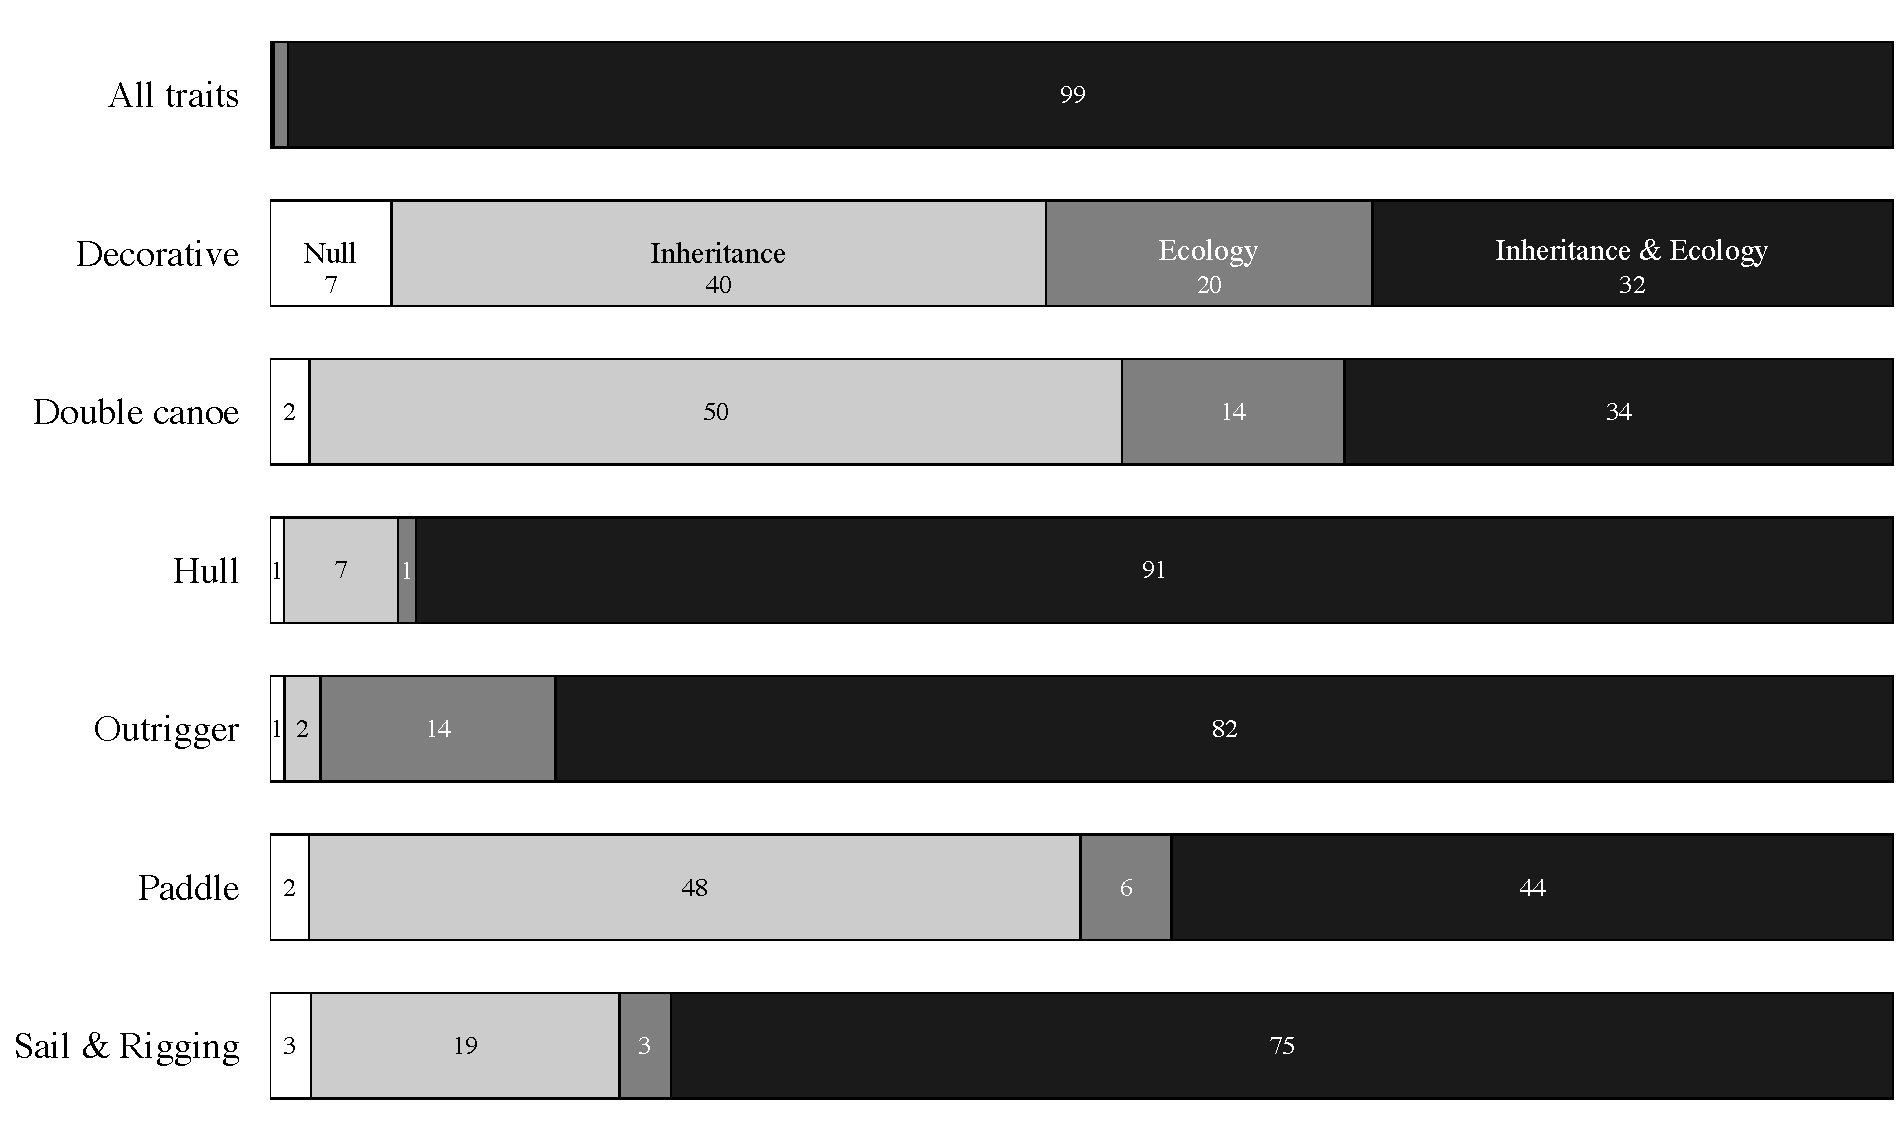
\includegraphics[scale=0.5]{figures/barplot.pdf}
  \end{center}
  \caption{Plot of the relative weight assigned to the four classes of models (where whitespace represents null models). Size of each colored region represents the sum of DIC weights attributed to that class of models, characterizing the relative weight of evidence in favor of that class of model \citep{Burnham&Anderson:2002}. The wider a specific region the more likely the corresponding class of models describes the process behind the evolution of that particular set of canoe traits. If no region is dominant, there is less certainly or the models explain very little.}
  \label{fig:barplot}
\end{figure}

We classify 65 distinct canoe traits for 11 island groups into six general categories: hull design, decoration, rigging, paddles, outrigger traits and double-hulled canoe traits (see ESM for details). DIC scores were calculated for each of the 27 models fitted to the full dataset, and separately fitted to each of the six trait subsets. Since these scores are only meaningful in relation to those of other models, a given model's absolute score is less important than its relative distance to the top model's score ($\Delta$ DIC) and the model's information criterion weight, $w$. The results of each analysis are presented in Figure \ref{fig:barplot}, which measures the relative explanatory power of models that included only ecological covariates (E), covariates of cultural inheritance (C), both (CE), and the two null models.

\begin{figure}[t]
  \begin{center}
    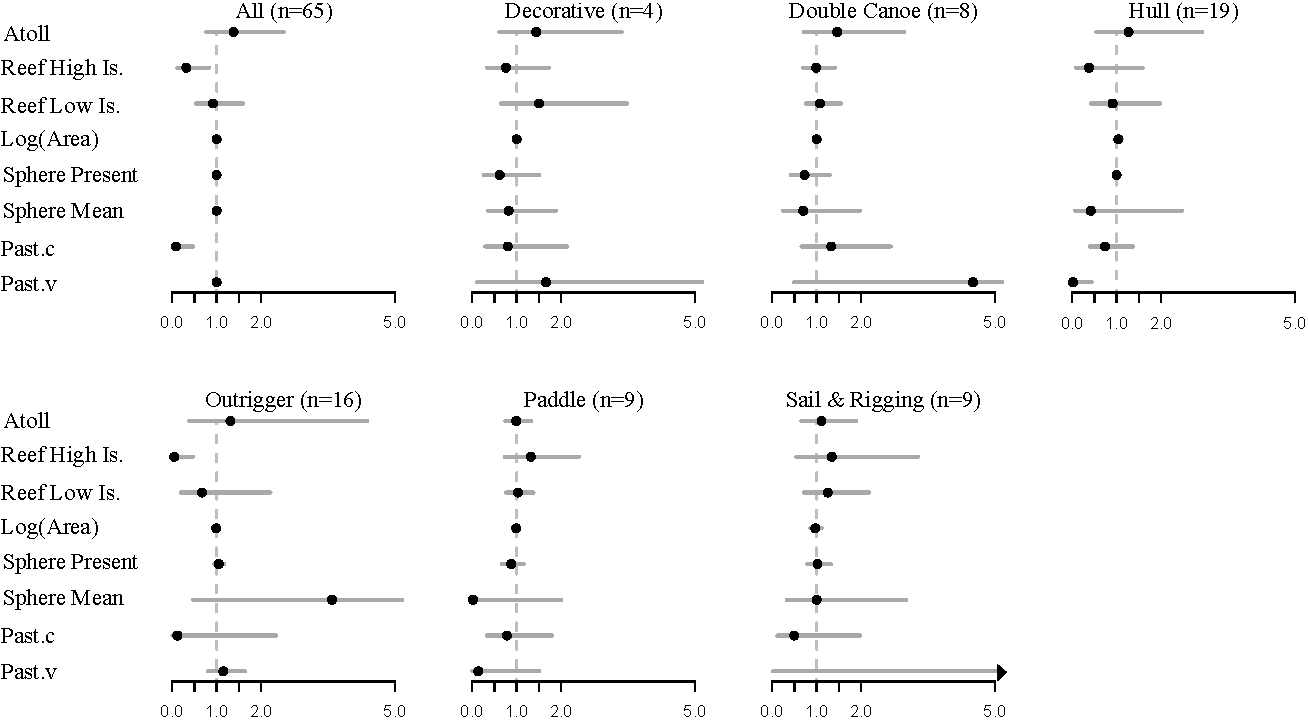
\includegraphics[scale=0.7]{figures/oddsratios.pdf}
  \end{center}
  \caption{Model-averaged odds-ratio estimates with 95\% Upper and Lower bounds for eight covariates. The first three covariates estimate the effects of modal properties of the island group; whether or not the islands are atolls, high islands with reefs or low islands with reefs. The remaining four covariates describe an island group's cultural ancestors and neighbors; ''sphere present'' and ''sphere mean'' consider the presence and frequency, respectively, of each canoe trait within trade interaction spheres, while ''past.c'' and ''past.v'' consider the presence of each canoe trait among island groups earlier in the settlement sequence, using constant or trait-varying imputed values, respectively, for the first island group in the sequence (see ESM).}
  \label{fig:oddsratios}
\end{figure}

\subsection{Model rankings}

Considering all canoe traits, models that include both cultural and ecological (CE) covariates consistently outperform those including either covariate category alone. When considering all 65 traits, the top four models, all CE, constitute 99\% of the total DIC weight. Among the CE class of models, those that consider island settlement sequence, island area, and geological type of island perform the best (see ESM). The top model with 67\% of the total weight considers only settlement sequence and island type. The second model at 27\% of the weight has the same covariates as the top model but with the addition of the log(area) covariate. Finally, the third ranking model adds trade spheres, though because its weight is only 4\%, post-settlement interactions between islands are less useful on average across these data.

This basic pattern is also found for traits specific to the canoe's hull, sail and rigging, and traits specific to outriggers; CE models of one form or another rank the highest and take up the majority of the model weights in each subcategory. The top model for hull traits, with 41\% of the model weight, includes settlement sequence, area, and island type. The next best (18\%) includes trading partners and drops island type, together covering all four covariate categories. Considering sail and rigging traits, CE models rank highest, but the top models carry roughly equal weight, indicating equivalent explanatory utility. For outrigger traits the top model at 42\% weighting includes island type and settlement sequence, and the second ranked model (26\%) adds log(area) and trading spheres. 

While models that include only cultural inheritance covariates occasionally outperform the composite CE models, though the same cannot be said for ecology models or the null models. These C models dominated the rankings for paddle traits (Figure~\ref{fig:barplot}), whose top model considers only settlement sequence and trading spheres, both present in nearly all models that outperformed the null. For double-hull canoe traits, C models take up the majority of model weights, though among them there is no clear winner. 

The models rankings for decorative traits are in contrast to those of all other trait subsets. The top two models consider only covariates of cultural inheritance, constituting 13\% and 11\% of model weight, respectively. However, the third ranking model, at 7\%, is the null model Base, followed by CE and E models all at around 6\% of model weight. In general the model weights for decorative traits are distributed among CE, C and E models roughly equally (Figure \ref{fig:barplot}). We interpret the inability to distinguish a clear winner and the prominence of the null model as evidence of poor performance among all our models, and so none are particularly compelling explanations the observed variation in canoe decoration \citep{Burnham&Anderson:2002}. 


\subsection{Effects of single covariates}

We also report model-averaged odds-ratios (see ESM for discussion on model-averaging methods). Primarily, the estimates reflect the uncertainty in predicting canoe traits using any one particular covariate (the dimensions of our sample are 11 islands by 65 traits, suggesting only sparse information). Most estimates have lower and upper bounds that include 1.0, the value of ``no effect'', though the posterior means of many estimates are far from one. However, while some covariates may have imprecise point estimates (broad posterior distributions), they do in many cases contribute to a model's performance in the above model rankings. Despite estimate uncertainty, model selection methods can still be used to make inferences. 

Some of the more precise and contrasting estimates are worth noting (Figure \ref{fig:oddsratios}). The ecological covariate ``Reef High Is.'', a dummy variable for this island profile, has a negative effect on all canoe traits taken together, and specifically outrigger and (more ambiguously) hull traits. In terms of the odds ratio, any given canoe trait is much less likely to be present on high, reefed islands than when island type is unknown. 

We also estimate strong negative predictive effects for settlement sequence covariates for a variety of canoe traits, meaning that they are less likely to be present on an island group if those traits are present or common in the ancestral region of the Pacific that settled that island group. Specifically, covariate ``Past.c'' has a negative predictive effect on canoe traits in general and a (more ambiguous) negative effect on outrigger traits. The other settlement sequence covariate, ``Past.v'', has a particularly strong negative effect on hull and paddle traits. (We consider the effect strong because the mean estimate is far from one and a relatively small portion of the total interval extends across one). We registered only two estimates of positive effect on the odds ratio, both ambiguous; settlement sequence (``Past.v'') on double canoe traits, and trading spheres (``Sphere mean'') on outriggers. 


\section{Discussion}

Taken together, these results tell an interesting story about Oceanic canoe designs. The majority of focal canoe traits are best explained by settlement sequence and island type; there is little to no evidence that island land area or inter-island trade enhances our understanding of canoe trait distribution. When clear, the estimated effects of settlement sequence and island type are also strongly negative - our models predict that the settlement of high, volcanic islands with reefs is followed by the disappearance of these canoe traits. This is particularly true for outrigger and hull designs.   

Exactly why the settlement of high, reefed islands is associated with the absence of our focal canoe traits is an open question. Of the eleven island groups considered, two of the largest (Hawaii and New Zealand) have the fewest canoe traits (24 and 23 traits, respectively, out of 65). However, Fiji, by land area larger than Hawaii, has 34 traits, one of the highest in the sample. As a result, while models including the log of island area are among the top ranked, the estimated effect of island area on the odds ratio is negligible.

Instead of land area, our high island covariate may be capturing the effects of greater natural resources available on high islands; Maori designs in New Zealand could use trees so massive double-hull and outrigger designs were no longer necessary, while canoe builders on low islands like the Tuamotos had to work with lashed planks in lieu of simple dugouts. Indeed, many of the focal canoe traits in our sample can be seen as adaptations to low-resource environments, and so it may be expected that these would be abandoned upon the ecological release of reaching Hawaii and New Zealand. 

Another possibility is the effects of population size on canoe design. \cite{Henrich2004:Tasmania} demonstrates how sampling error in low population sizes can cause the decay and eventual disappearance of useful technology, such as observed on Tasmania. The process on New Zealand and Hawaii may be roughly the opposite - massive technological undertakings that require state-like centralized political authority and the collective knowledge of large networks of canoe designers may rapidly replace technological designs that can be sustained within smaller founding populations. 

Both hypotheses imply that a key influence on the results is the processes about \textit{which} canoe traits are recorded and coded. This is a important methodological point, as two subsequent analyses \citep{RogersFeldmanEhrlich2009,GrayBryantGreenhill2010} have been carried out on the \cite{Rogers2008:Canoes} dataset, and the results of each may be sensitive to alternative coding. From the descriptions of Haddon and Hornell, among others, New Zealand and Hawaii clearly do not have a dearth of canoe designs. However, because the focus of anthropological analysis is the flow of canoe designs across Polynesia, variations in canoe technology unique to these end-sequence islands groups may be underrepresented in the analyses. Using our methods, future work that includes a greater emphasis on the diversity of canoe technology on high volcanic islands, as influenced by population size and natural resource constraints, should be able to provide an answer on this issue.

Though there are good theoretical reasons to think these methods reliably extract information from the data at hand, those results must be evaluated in light of prior knowledge about the historical record. Since there is strong evidence from oral histories that shunting-capable sailing rigs spread from Fiji through a settled Polynesia, the fact our models do not nominate inter-island trade in the ``sail and rigging'' analysis may say more about our sample and coding procedures than the actual diffusion of canoe technology. Likewise, other covariates that better capture neutral drift and the dynamics of ethnic markers may prove to be more effective at explaining the distribution of decorative traits. 

Despite these reservations, our results present clear quantitative evidence that statistical models incorporating both ecological and cultural inheritance covariates are better explanations of Oceanic canoe designs than either alone. Moreover, using these methods we are able to elucidate interesting patterns in the historical record without arguing for or against particular evolutionary processes. Our analysis provides support for the inclusion of both social-historical and ecological perspectives in the study of Polynesian seafaring, and demonstrates a method by which historians and anthropologists can test hypotheses of cultural change through the direct comparison of formalized statistical models. 

\bibliographystyle{plainnat}
\bibliography{references}

\end{document}




























